\documentclass{beamer}
\usetheme{LANL}
\usepackage{beamer_defaults}

\title[Sample]{~ \\ \vspace{5pt}Sample Beamer Presentation \\ ~}
\author[Jibben]{Z. Jibben}
\institute[ASU]{
  Arizona State University\\
  {\upshape Tempe, AZ} }
\date[\DTMsetup{datesep=.}\DTMsetstyle{mmddyy}\today]{\today}

\begin{document}
\begin{frame}[noframenumbering]
  \maketitle
\end{frame}
% ===================================================================================================
\begin{frame}{Introduction}
  
  \begin{itemize}
  \item This is an example slide
  \item Recall the momentum equation
    \begin{equation*}
      \Dpart{\v{u}}{t} + \v{u}\cdot\nabla\v{u} = -\frac{1}{\rho}\nabla p +
      \frac{1}{\rho}\nabla\cdot(\mu(\nabla\v{u}+\nabla^\mathrm{T}\v{u})) + \v{g}
    \end{equation*}
  \end{itemize}
  
  \vspace{-3ex}
  \figbox{Discretization Comparison}{
    \centering
    \begin{subfigure}{0.3\textwidth}\centering
      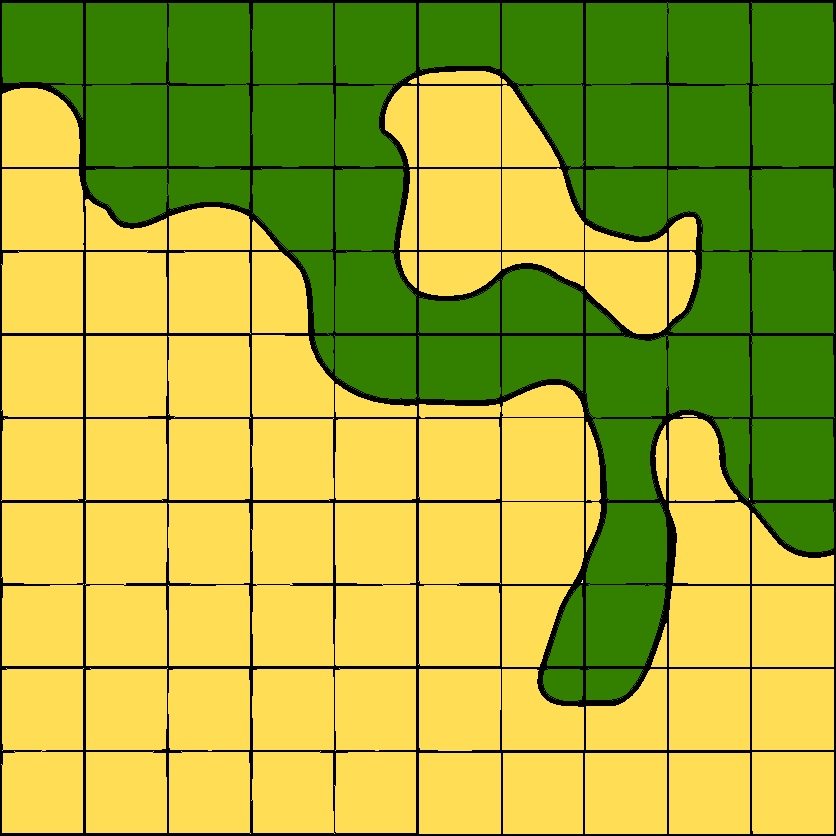
\includegraphics[width=0.9\textwidth]{interface}\hspace{5pt}
      \caption{interface}
    \end{subfigure}
    \begin{subfigure}{0.3\textwidth}\centering
      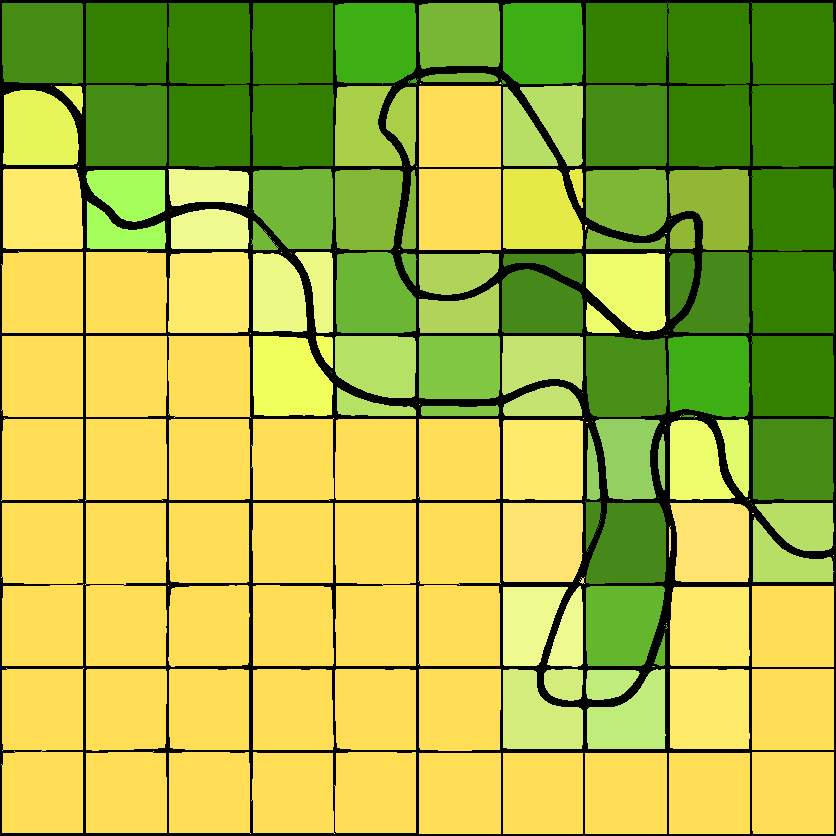
\includegraphics[width=0.9\textwidth]{interface_FV}\hspace{5pt}
      \caption{finite volume}
    \end{subfigure}
    \begin{subfigure}{0.3\textwidth}\centering
      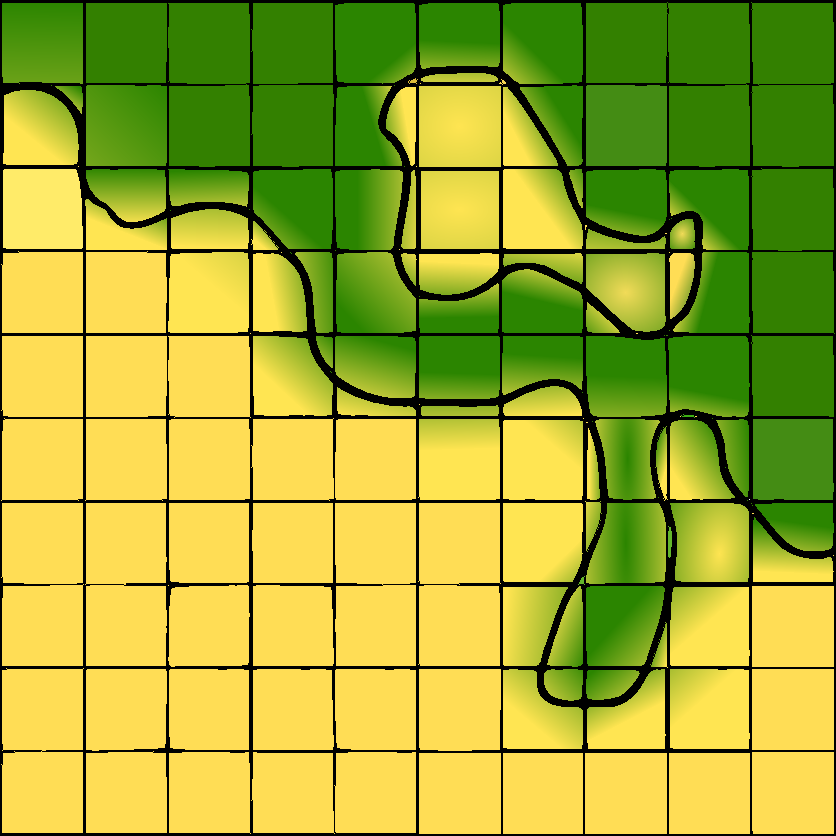
\includegraphics[width=0.9\textwidth]{interface_DG}
      \caption{DG}
    \end{subfigure}
  }
  
\end{frame}
\end{document}

%%% Local Variables:
%%% mode: latex
%%% TeX-master: t
%%% End:
